\headline{{\textbf{\Large\sffamily The Top Chop:}}\\
          {\textbf{\large\sffamily The Tree of the Month Contest}}}
\label{2025-10-contest}
\noindent
October's meeting unfurled a festival of colour that could rival any autumn woodland.
Our benches were aglow with fiery reds, glowing ambers, and mellow golds, as members interpreted this month's evocative theme: \textit{``Autumn Colours, Any Tree''}.
The variety was nothing short of inspiring --- from delicate deciduous leaves in transition to rugged evergreens showing hints of seasonal warmth.
The air was filled with quiet admiration, the rustle of leaves, and the appreciative murmurs of fellow enthusiasts who know just how fleeting --- and magical --- this time of year can be.

Each month, members bring forward one tree to compete for the title of Tree of the Month, while novice members may enter more than one, with only their highest score counted.
Judging is carried out anonymously by peers, excluding the tree's owner, with marks awarded for trunk, branch structure, foliage, pot choice, and interpretation of the theme --- up to 12 points per judge.

Normally, the committee collates and publishes the detailed scores for posterity (and a bit of friendly rivalry), but this month's results seem to have taken a small detour on their way to the newsletter --- perhaps lost in translation between clipboard and keyboard!
Rest assured, every vote has been logged with the usual care and precision by our ever\--diligent committee.
We may not have the full tally to pore over this month, but we do have our winners --- and what a splendid lineup they make.

\medskip
\topic{Tree of the Month}
\noindent
This month's table was a vivid celebration of autumn's brilliance, with each entry capturing the season's fleeting grace in its own way.
Here are the trees that graced our benches, listed alphabetically by the artist's surname:

\begin{enumerate}
    \item \textbf{Ryan Best} --- Yew (\textit{Taxus Baccata})
    \item \textbf{Chris Durne} --- Forsythia (\textit{Forsythia Intermedia})
    \item \textbf{David Fishwick} --- Hornbeam (\textit{Carpinus Betulus})
    \item \textbf{Brendan Gibbs} --- Cotoneaster (\textit{Cotoneaster Horizontalis})
    \item \textbf{Grant Kinnaird} --- Crabapple (\textit{Malus Sylvestris})
    \item \textbf{Nick Lloyd} --- Ginkgo Biloba (\textit{Ginkgo Biloba})
    \item \textbf{Tina Todd} --- Willow\--Leaved Cotoneaster (\textit{Cotoneaster Salicifolius})
    \item \textbf{Tony Ulatowski} --- Korean Hornbeam (\textit{Carpinus Turczaninowii})
    \item \textbf{Terry Wilson} --- Boston Ivy (\textit{Parthenocissus Tricuspidata})
\end{enumerate}

\noindent
Our warmest congratulations go to \textbf{Tony Ulatowski}, whose elegant Korean Hornbeam claimed top honours this month.
His tree displayed a painterly progression of colours --- rusted reds melting into soft golds --- all balanced with a graceful, mature silhouette.
% It was a vision of autumn distilled into living form: subtle yet striking, with each leaf a brushstroke of seasonal beauty.
% Tony's mastery of proportion and gentle refinement of branch structure were much admired, setting a high bar for future entries.

% While the other competitors may not have claimed the top spot, their contributions filled the room with inspiration.
% \textbf{Nick Lloyd}'s \textit{Ginkgo Biloba} offered a textbook example of that species' fan\--shaped leaves shifting from bright lime to buttery yellow;
% \textbf{Grant Kinnaird}'s \textit{Crabapple} carried clusters of glowing fruit that seemed to echo the fading sun;
% and \textbf{Tina Todd}'s \textit{Willow\--Leaved Cotoneaster} shimmered with fiery tones that hinted at both delicacy and strength.
% The diversity of forms, colours, and textures reflected not only the variety of the trees but also the diversity of vision within our club --- a reminder of how personal and expressive bonsai artistry can be.

\medskip
\topic{Novice Tree of the Month}
\noindent
Autumn's charm wasn't confined to the main contest.
Our Novice category this month was equally full of life and colour, proving that skill and sensitivity to the seasons begin early in one's bonsai journey.
Here are the entries, listed alphabetically by surname:

\begin{enumerate}
    \item \textbf{Dante Martini} --- Pine (\textit{Pinus Cembra?})
    \item \textbf{Gary Nichols} --- Hawthorn (\textit{Crataegus Monogyna})
    \item \textbf{Martin Redfern} --- Larch (\textit{Larix Decidua})
    \item \textbf{Anne\--Marie Weir} --- Dawn Redwood (\textit{Metasequoia Glyptostroboides})
\end{enumerate}

\noindent
First place in the Novice category goes to \textbf{Martin Redfern} for his graceful \textit{Larch}, which perfectly embodied the spirit of the season.
The tree's slender needles, turning from soft green to brilliant gold, evoked the transience of autumn's glory --- a poignant reminder that beauty often lies in transformation.
% The subtle taper of the trunk and the careful spacing of branches revealed both thoughtful design and patient care, qualities that mark Martin as one to watch in the coming months.

% Our other novice entrants also deserve heartfelt applause.
% \textbf{Dante Martini}'s \textit{Pine} brought an alpine crispness to the display, while \textbf{Gary Nichols}' \textit{Hawthorn} showed early signs of maturity with its rugged bark and gentle movement.
% \textbf{Anne\--Marie Weir}'s \textit{Dawn Redwood} was a graceful newcomer, capturing attention with its fine texture and warm autumnal blush.
% Each novice tree told a story of learning, experimentation, and quiet devotion --- the hallmarks of a bonsai artist in the making.

\medskip
\noindent
With October's contest concluded, we extend our thanks to everyone who brought their trees and enthusiasm to the evening.
Even without the usual spread of scores to debate and dissect, the atmosphere was rich with appreciation and good humour --- proof that the spirit of the competition lies not just in numbers but in shared passion and craftsmanship.
Next month's theme, \textit{``Any Tree Previously Submitted for Tree of the Month During the Year''}, invites members to revisit their favourites, refine their compositions, and perhaps even turn past entries into new triumphs.

\medskip
\noindent
So as the days shorten and the leaves fall, remember: every branch carries a story, every root holds a season's memory, and every tree --- whether award\--winning or simply admired --- keeps the art of bonsai alive.
Until next time, keep shaping, keep growing, and keep your passion evergreen.

\begin{center}
    \begin{minipage}[b]{.4\columnwidth}
        
\includegraphics[angle=0,origin=c,width=1.0\textwidth]{2025_10/res/contest_01_winner}
    \end{minipage}\quad
    \begin{minipage}[b]{.4\columnwidth}
        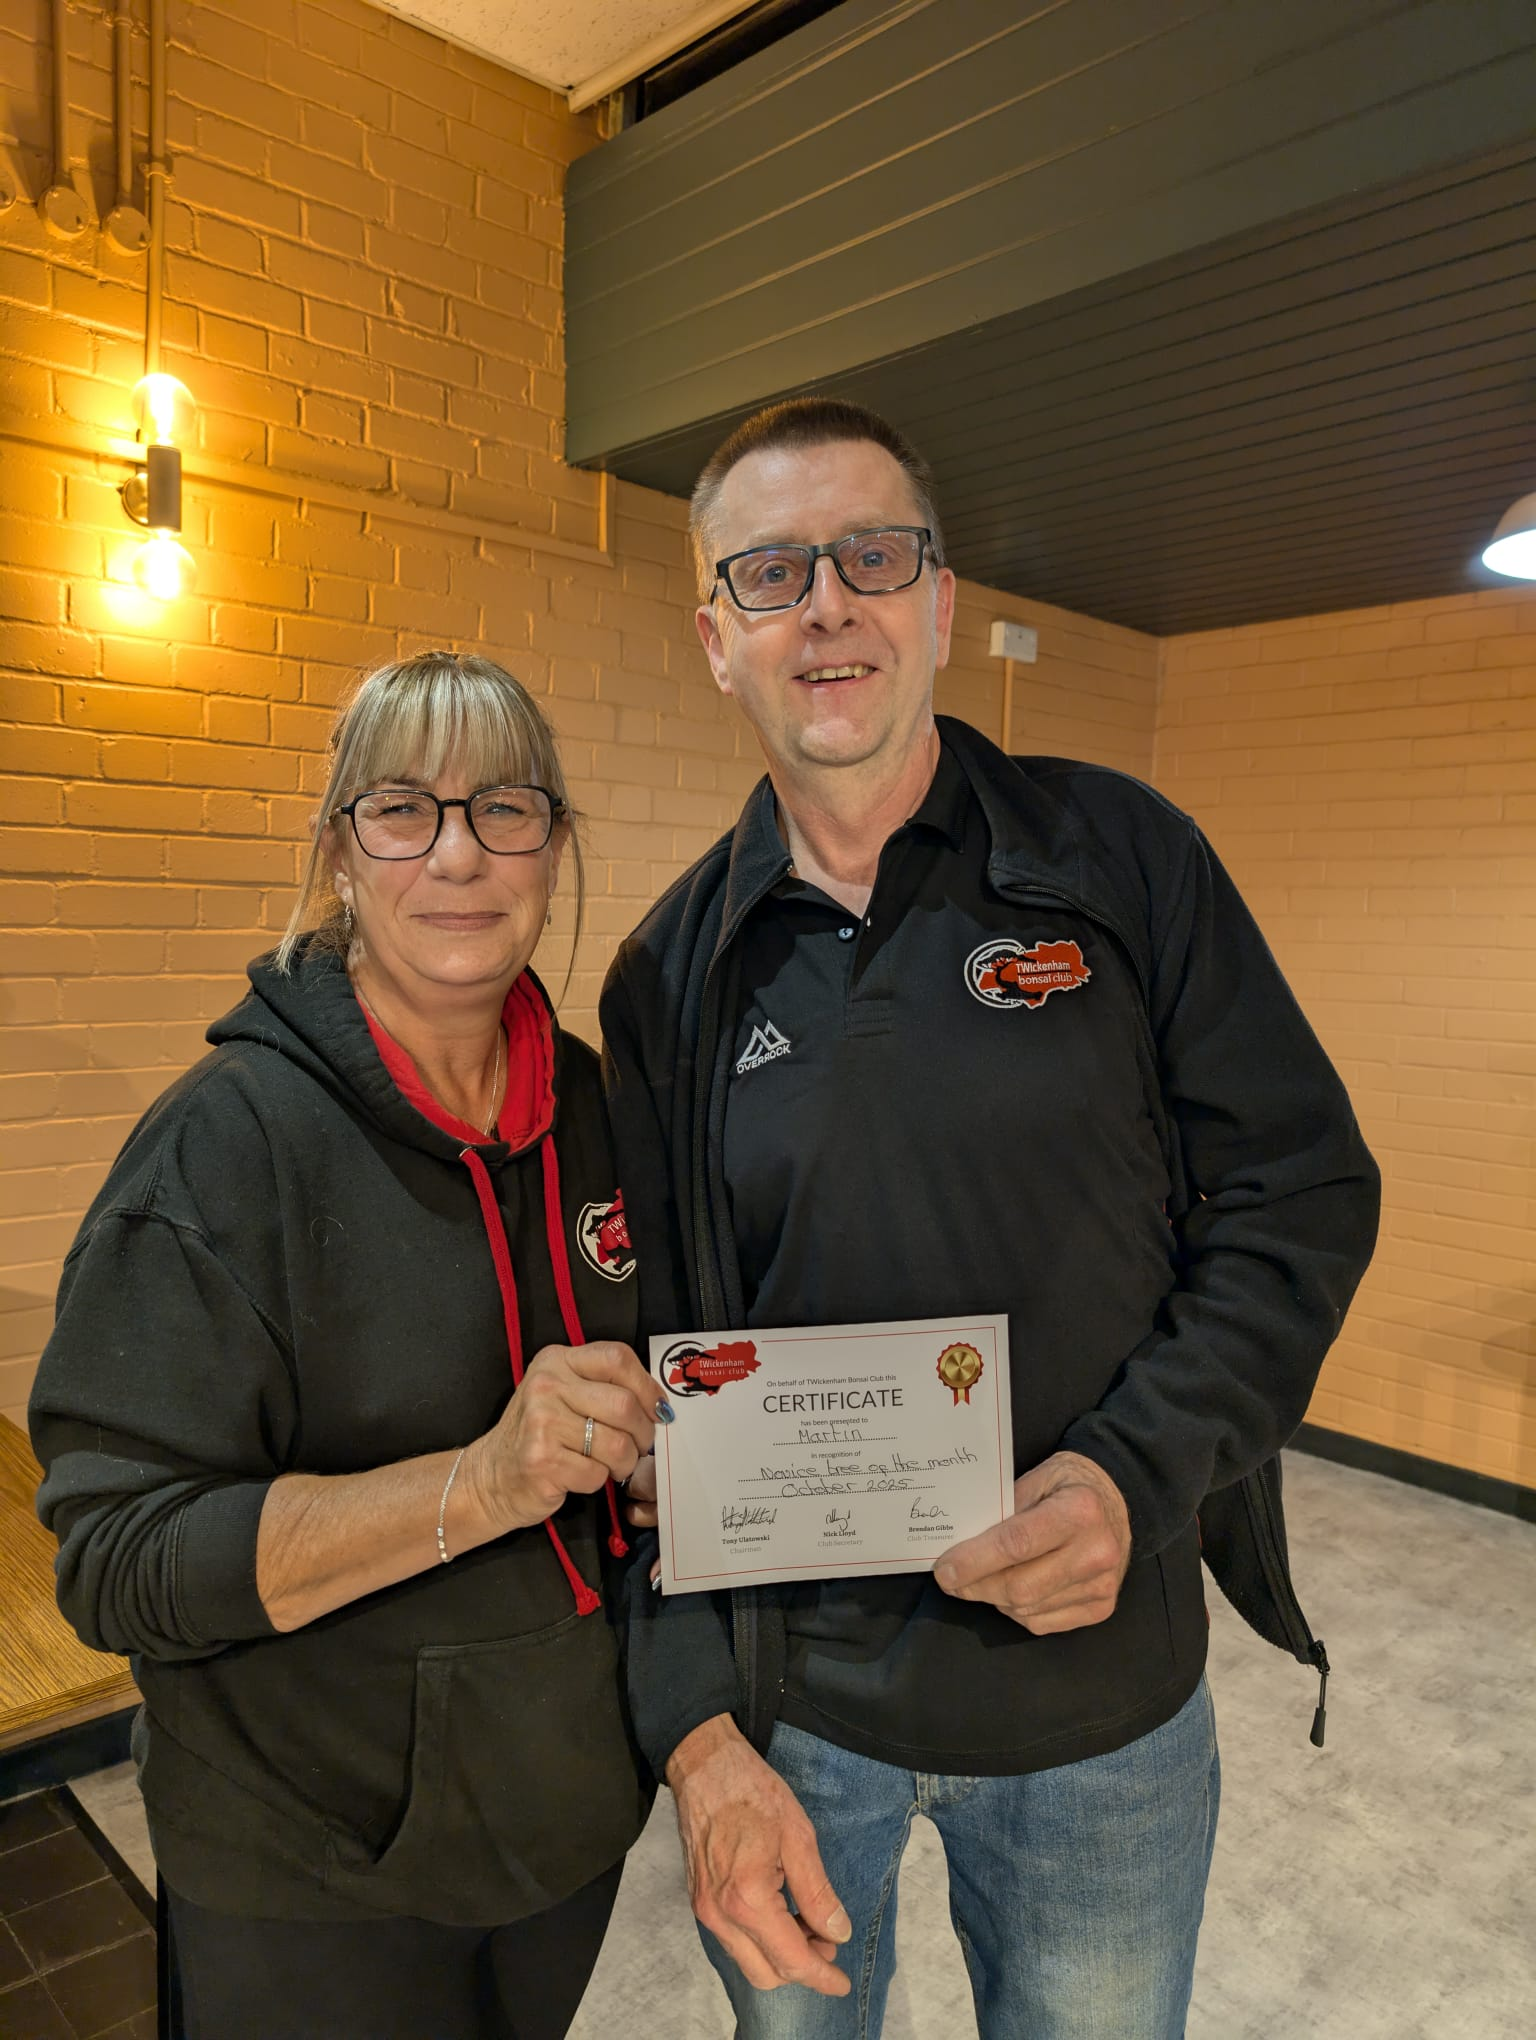
\includegraphics[angle=0,origin=c,width=1.0\textwidth]{2025_10/res/contest_02_winner}
    \end{minipage}
\end{center}

\closearticle

\end{multicols}

\begin{center}
    \begin{minipage}[b]{.275\textwidth}
        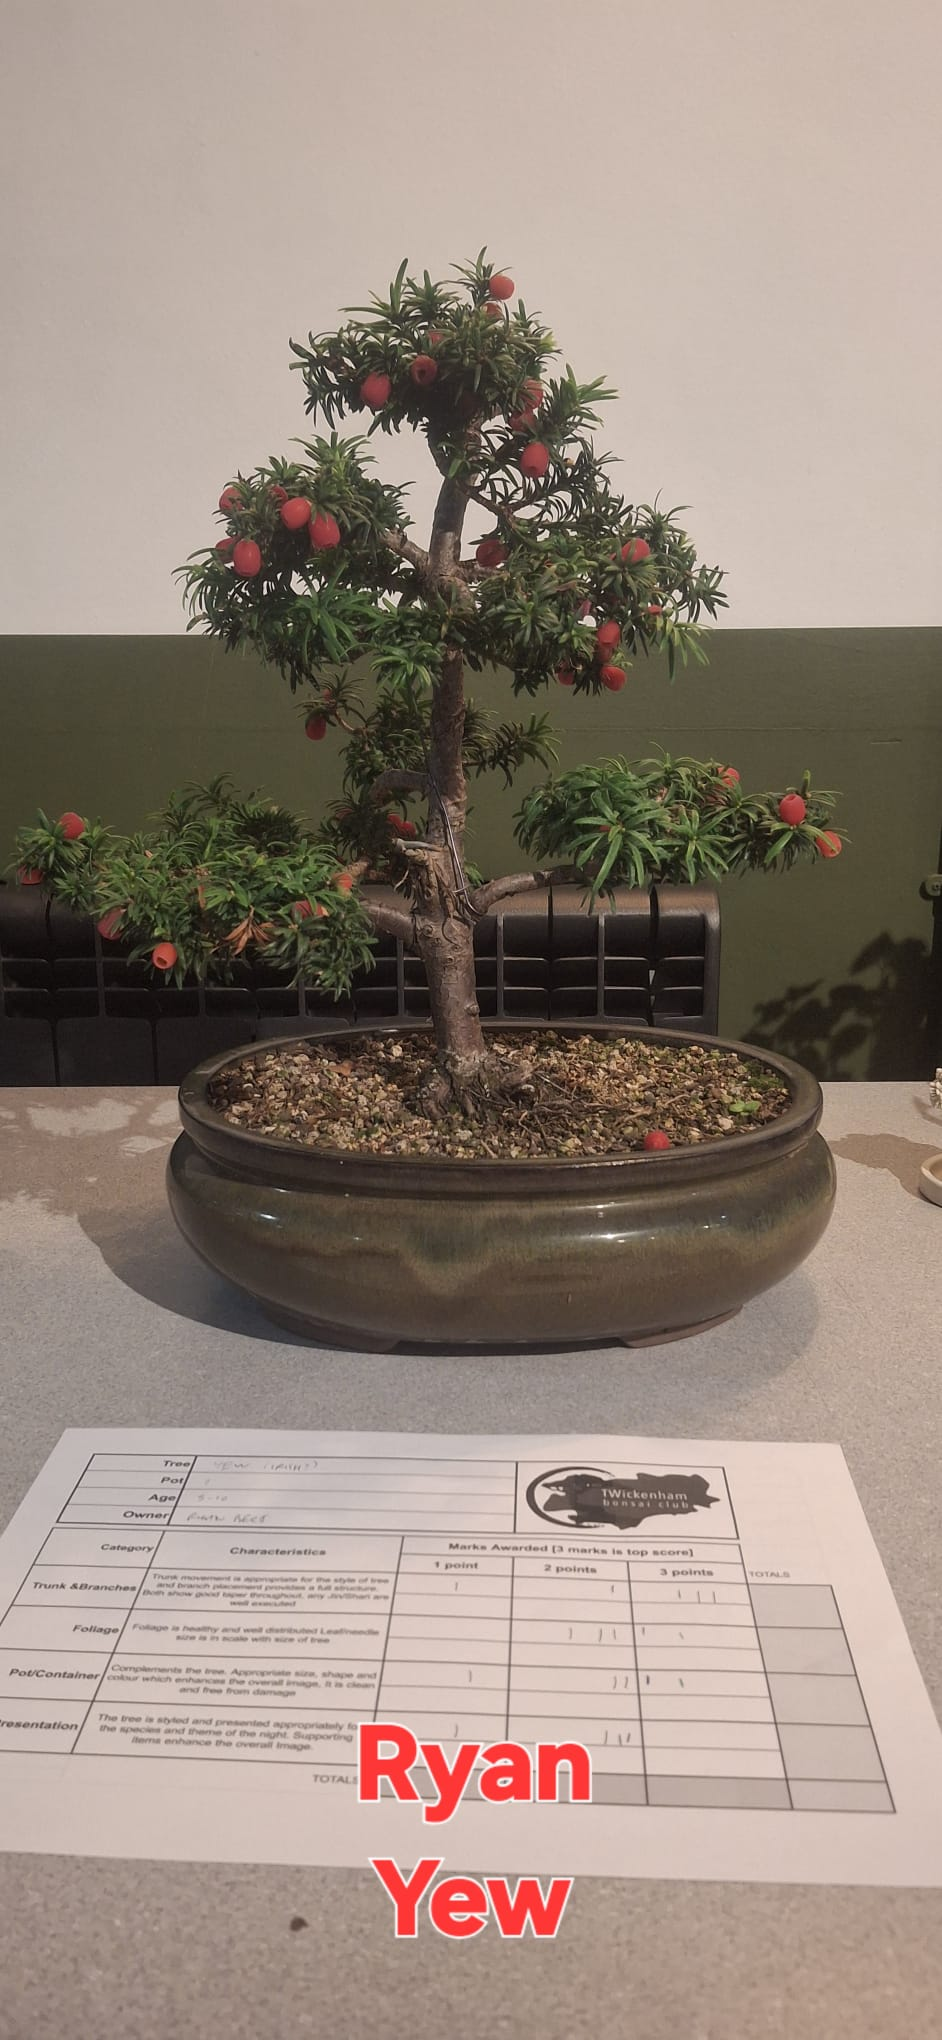
\includegraphics[angle=0,origin=c,width=1.0\textwidth]{2025_10/res/contest_ryan_best_yew}
        \centerline{\emph{Ryan Best's Yew}}
    \end{minipage}\quad
    \begin{minipage}[b]{.275\textwidth}
        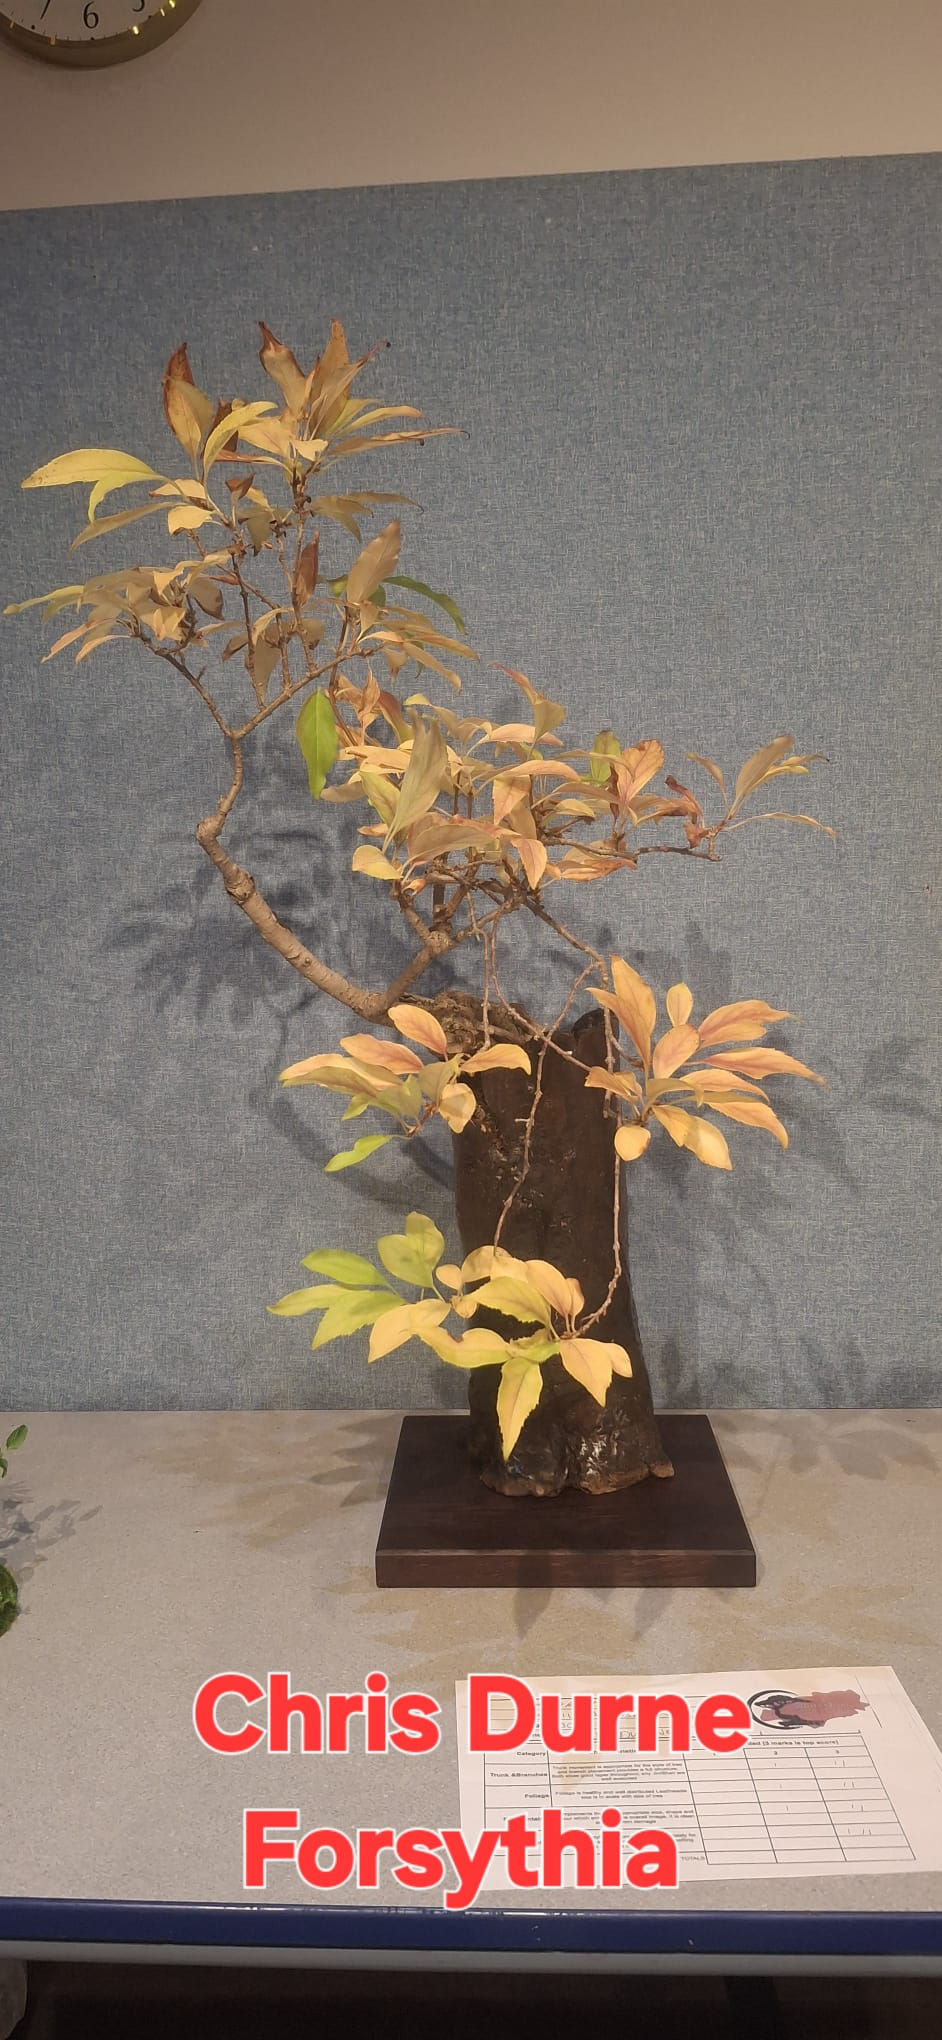
\includegraphics[angle=0,origin=c,width=1.0\textwidth]{2025_10/res/contest_chris_durne_forsythia}
        \centerline{\emph{Chris Durne's Forsythia}}
    \end{minipage}\quad
    \begin{minipage}[b]{.275\textwidth}
        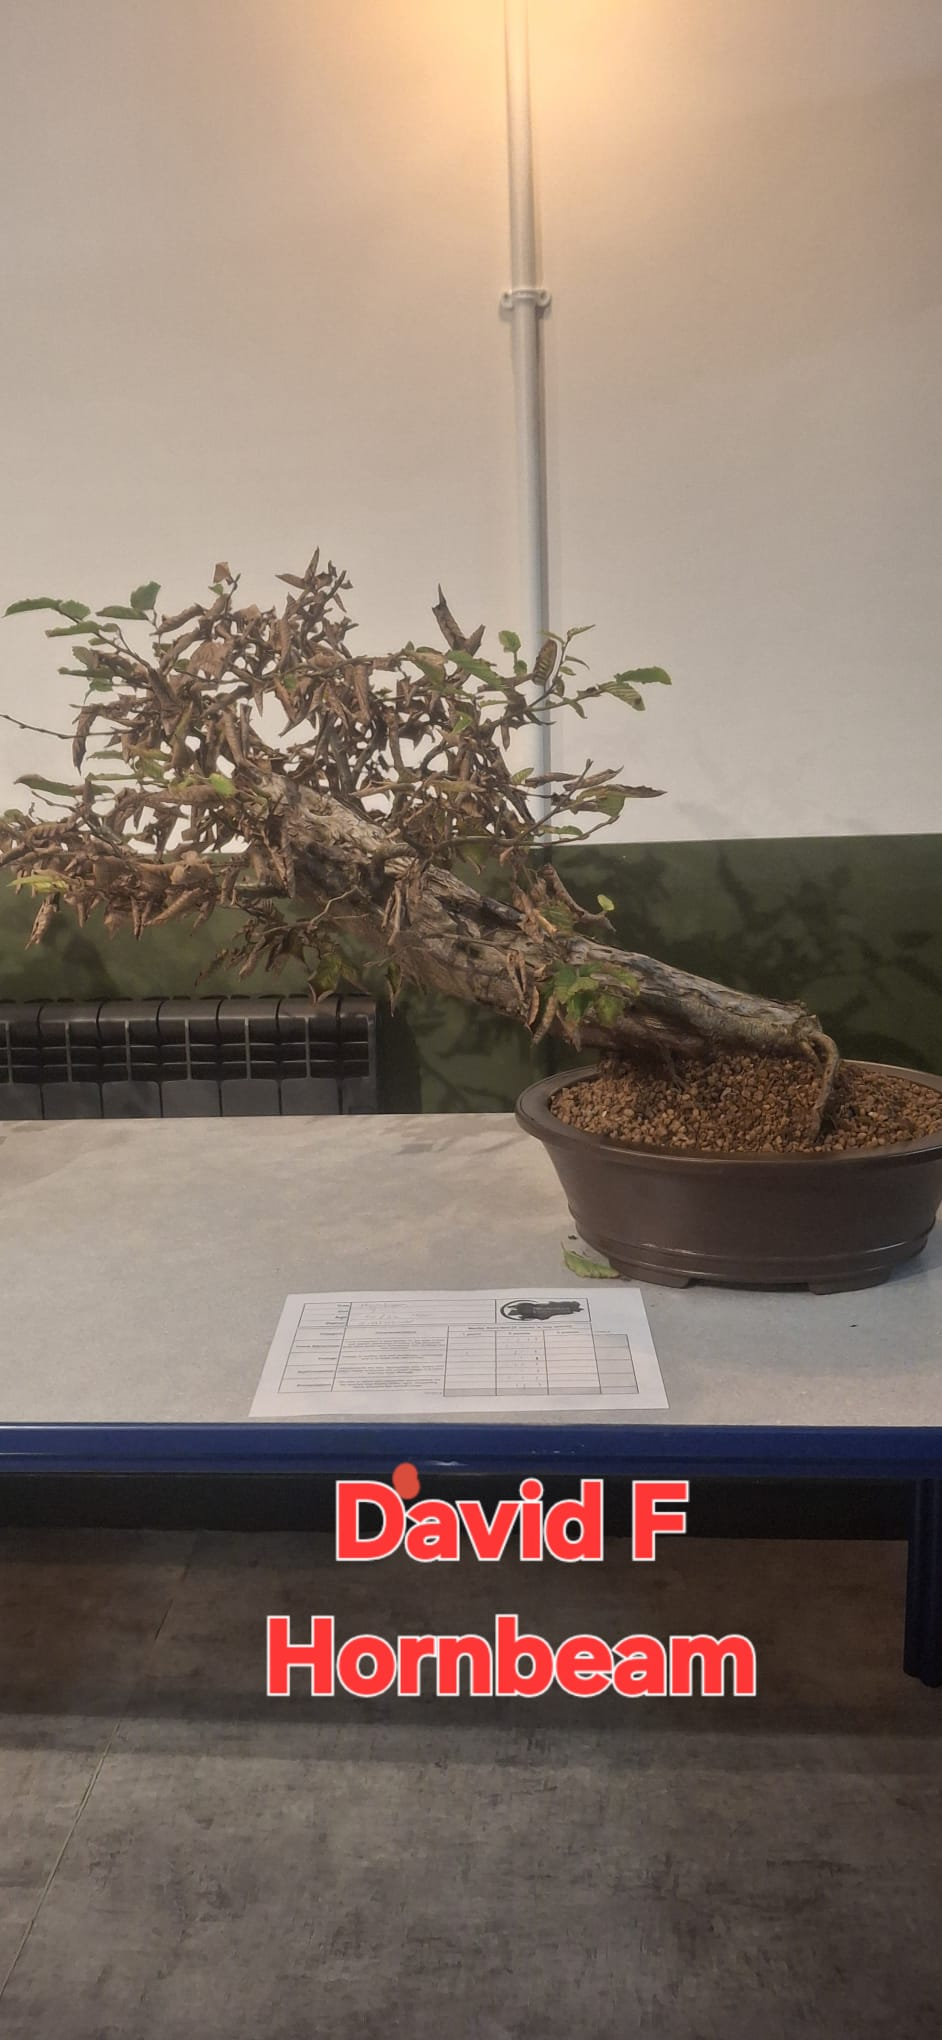
\includegraphics[angle=0,origin=c,width=1.0\textwidth]{2025_10/res/contest_david_fishwick_hornbeam}
        \centerline{\emph{David Fishwick's Hornbeam}}
    \end{minipage}
    \medskip

    \begin{minipage}[b]{.275\textwidth}
        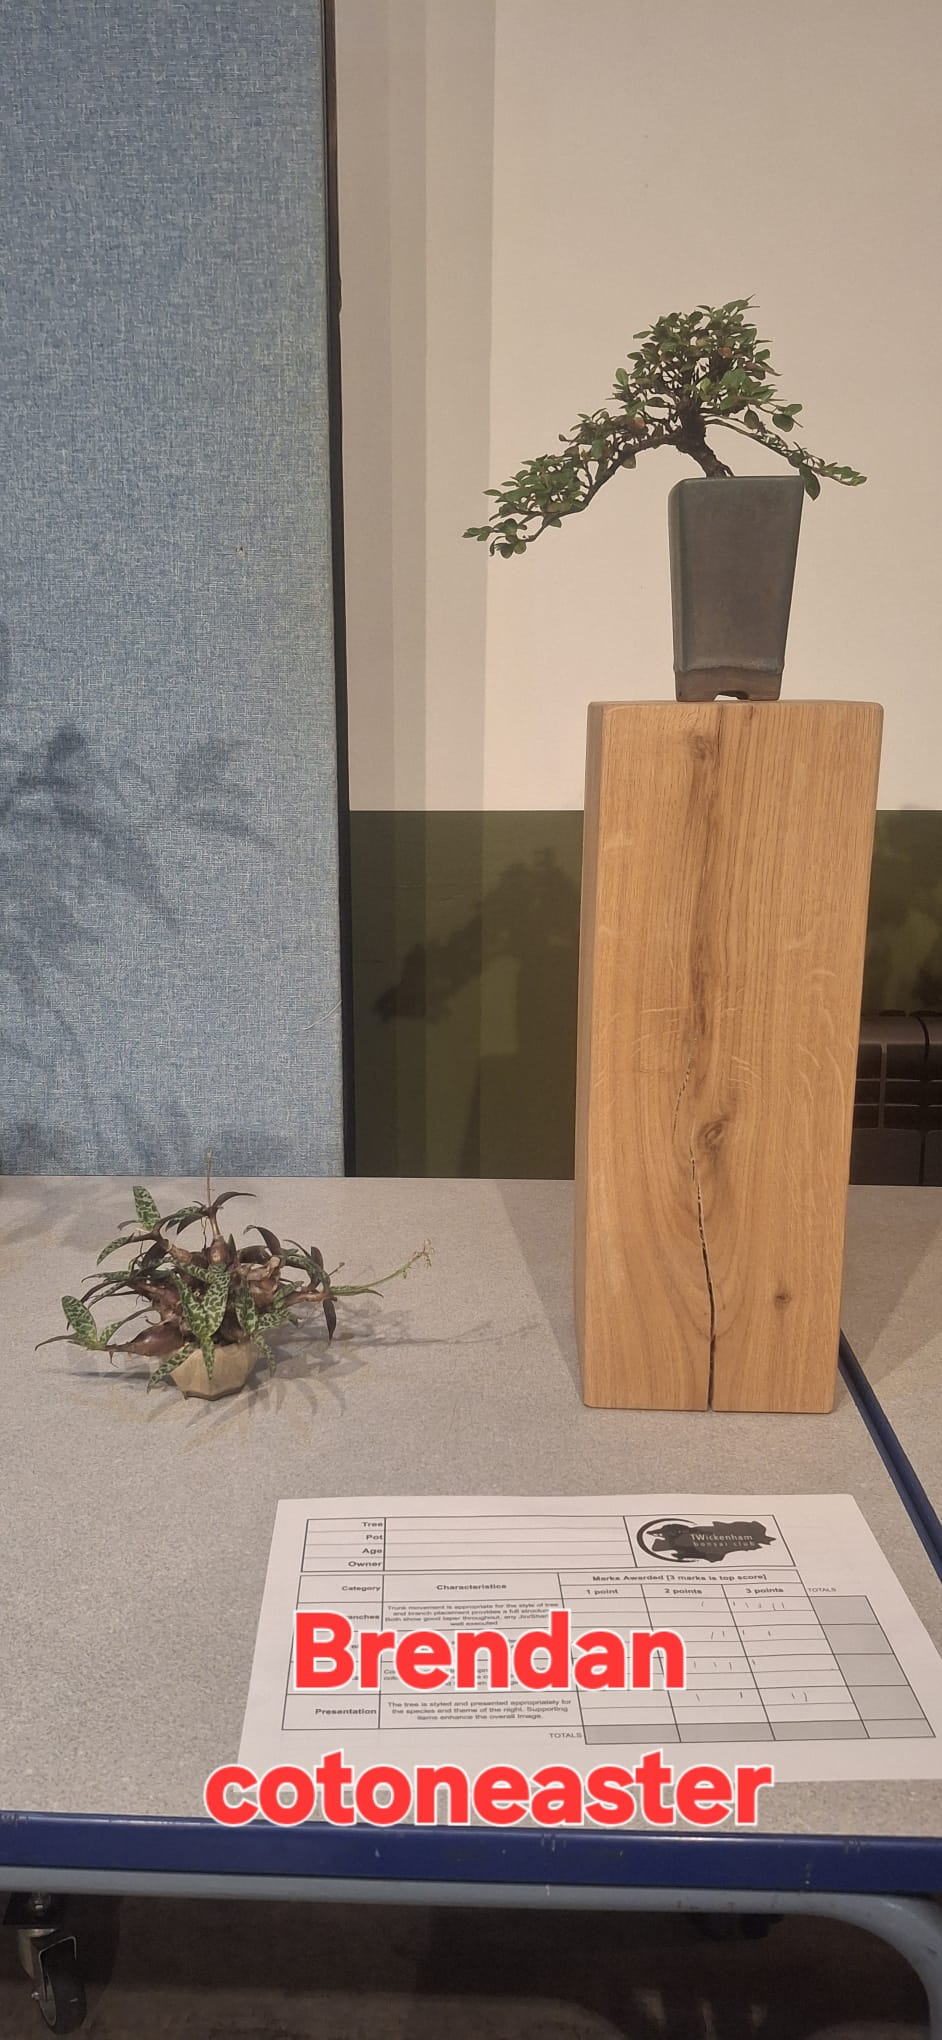
\includegraphics[angle=0,origin=c,width=1.0\textwidth]{2025_10/res/contest_brendan_gibbs_cotoneaster}
        \centerline{\emph{Brendan Gibbs' Cotoneaster}}
    \end{minipage}\quad
    \begin{minipage}[b]{.275\textwidth}
        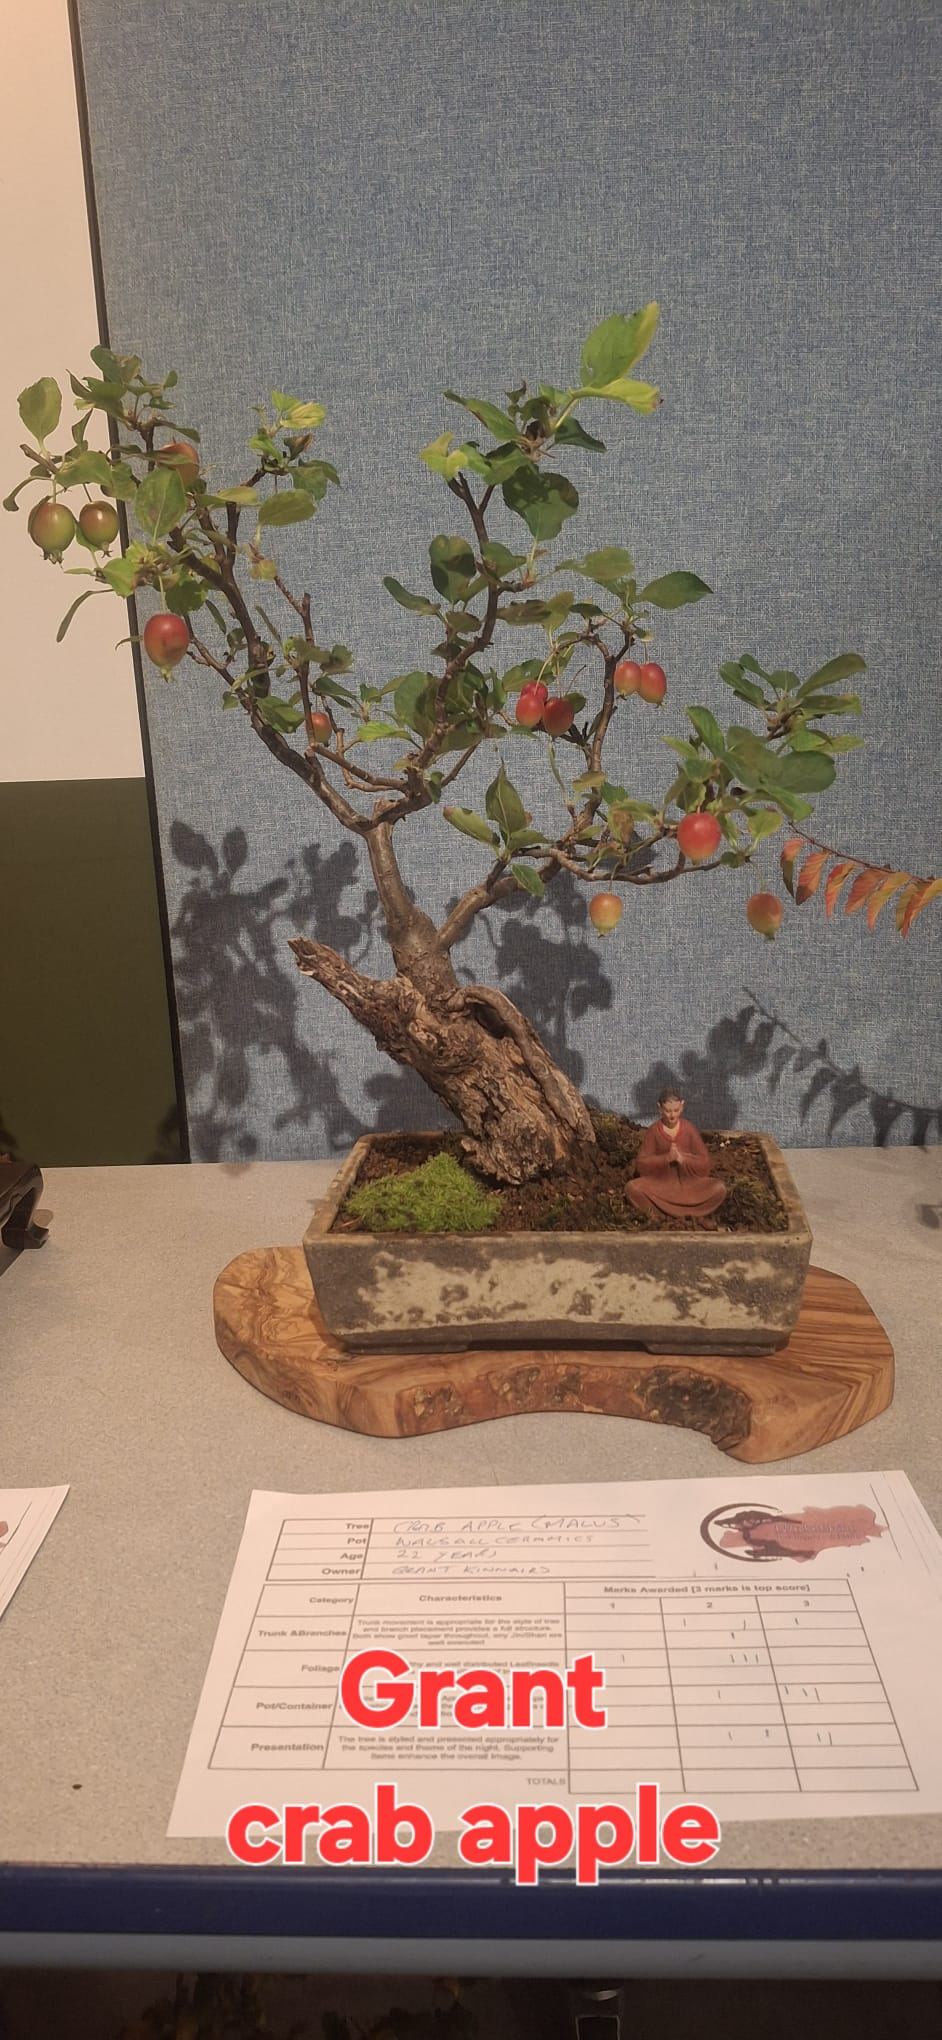
\includegraphics[angle=0,origin=c,width=1.0\textwidth]{2025_10/res/contest_grant_kinnaird_crab_apple}
        \centerline{\emph{Grant Kinnair's Crab Apple}}
    \end{minipage}\quad
    \begin{minipage}[b]{.275\textwidth}
        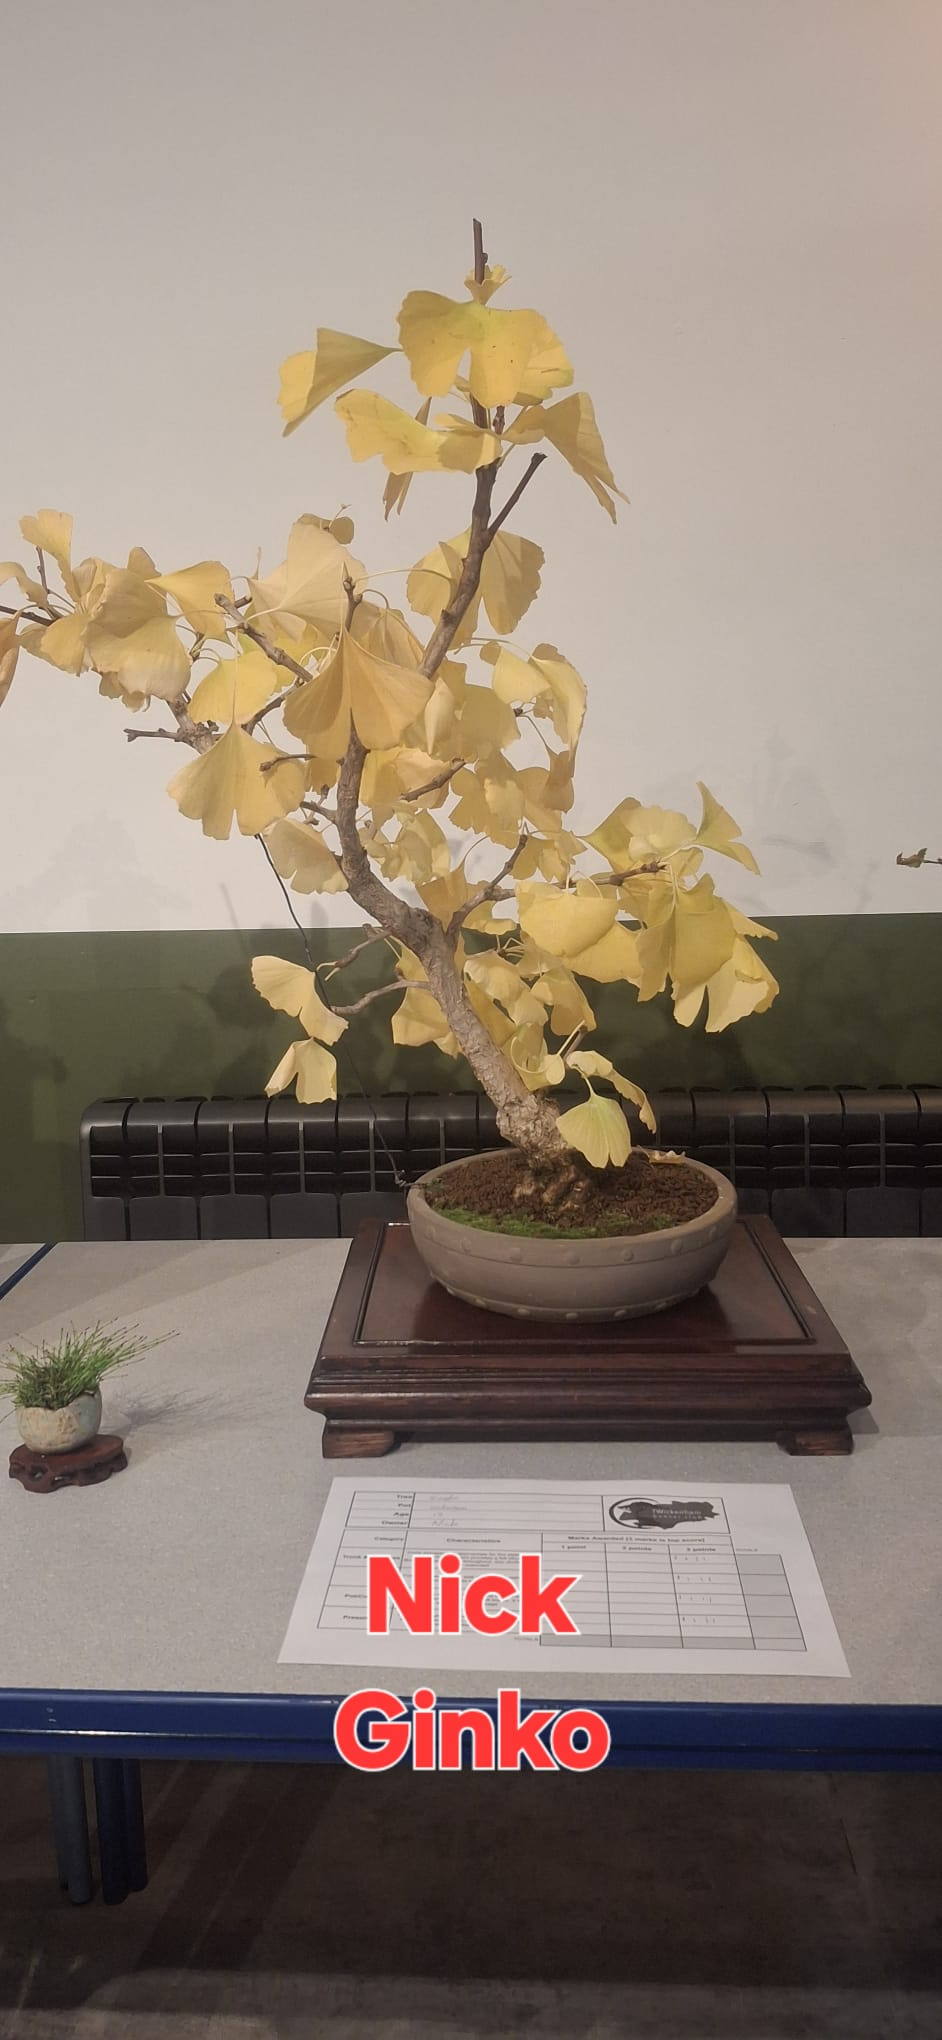
\includegraphics[angle=0,origin=c,width=1.0\textwidth]{2025_10/res/contest_nick_lloyd_ginkgo}
        \centerline{\emph{Nick Lloyd's Ginkgo}}
    \end{minipage}
\end{center}
\clearpage

\begin{center}
    \begin{minipage}[b]{.275\textwidth}
        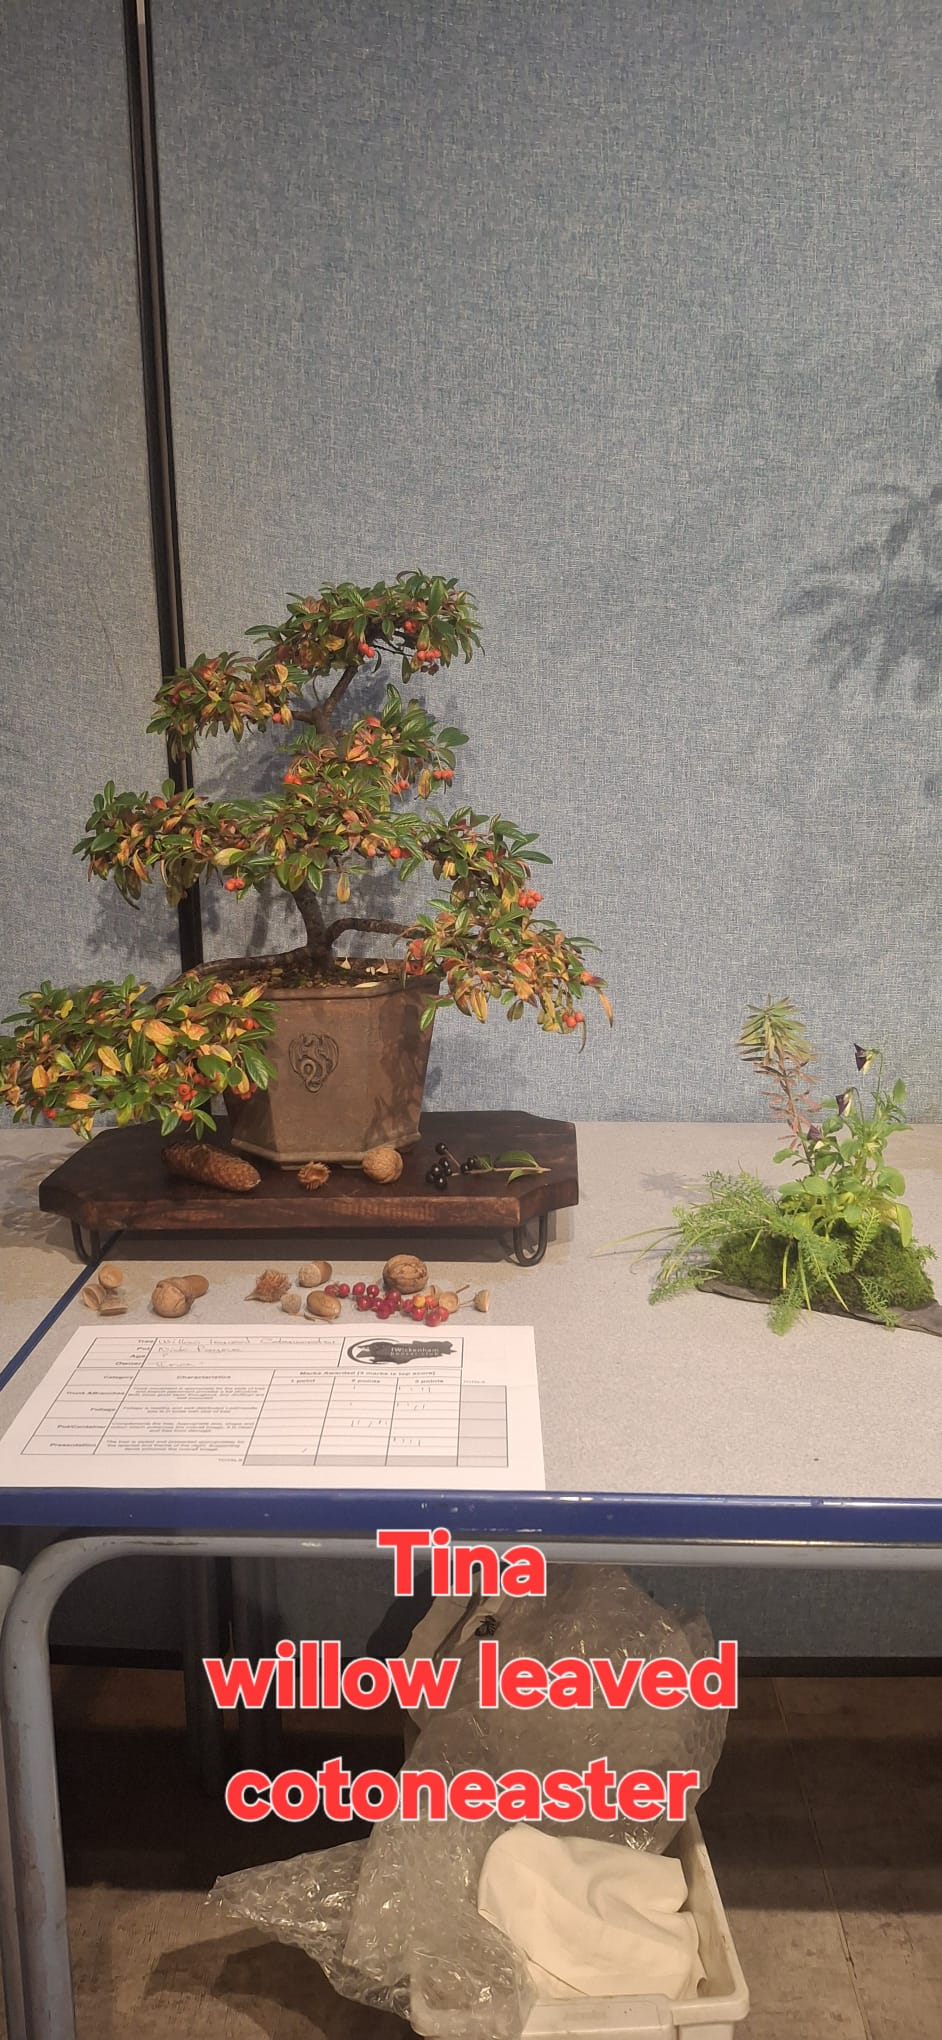
\includegraphics[angle=0,origin=c,width=1.0\textwidth]{2025_10/res/contest_tina_todd_willow_leaved_cotoneaster}
        \centerline{\emph{Tina Todd's Cotoneaster}}
    \end{minipage}\quad
    \begin{minipage}[b]{.275\textwidth}
        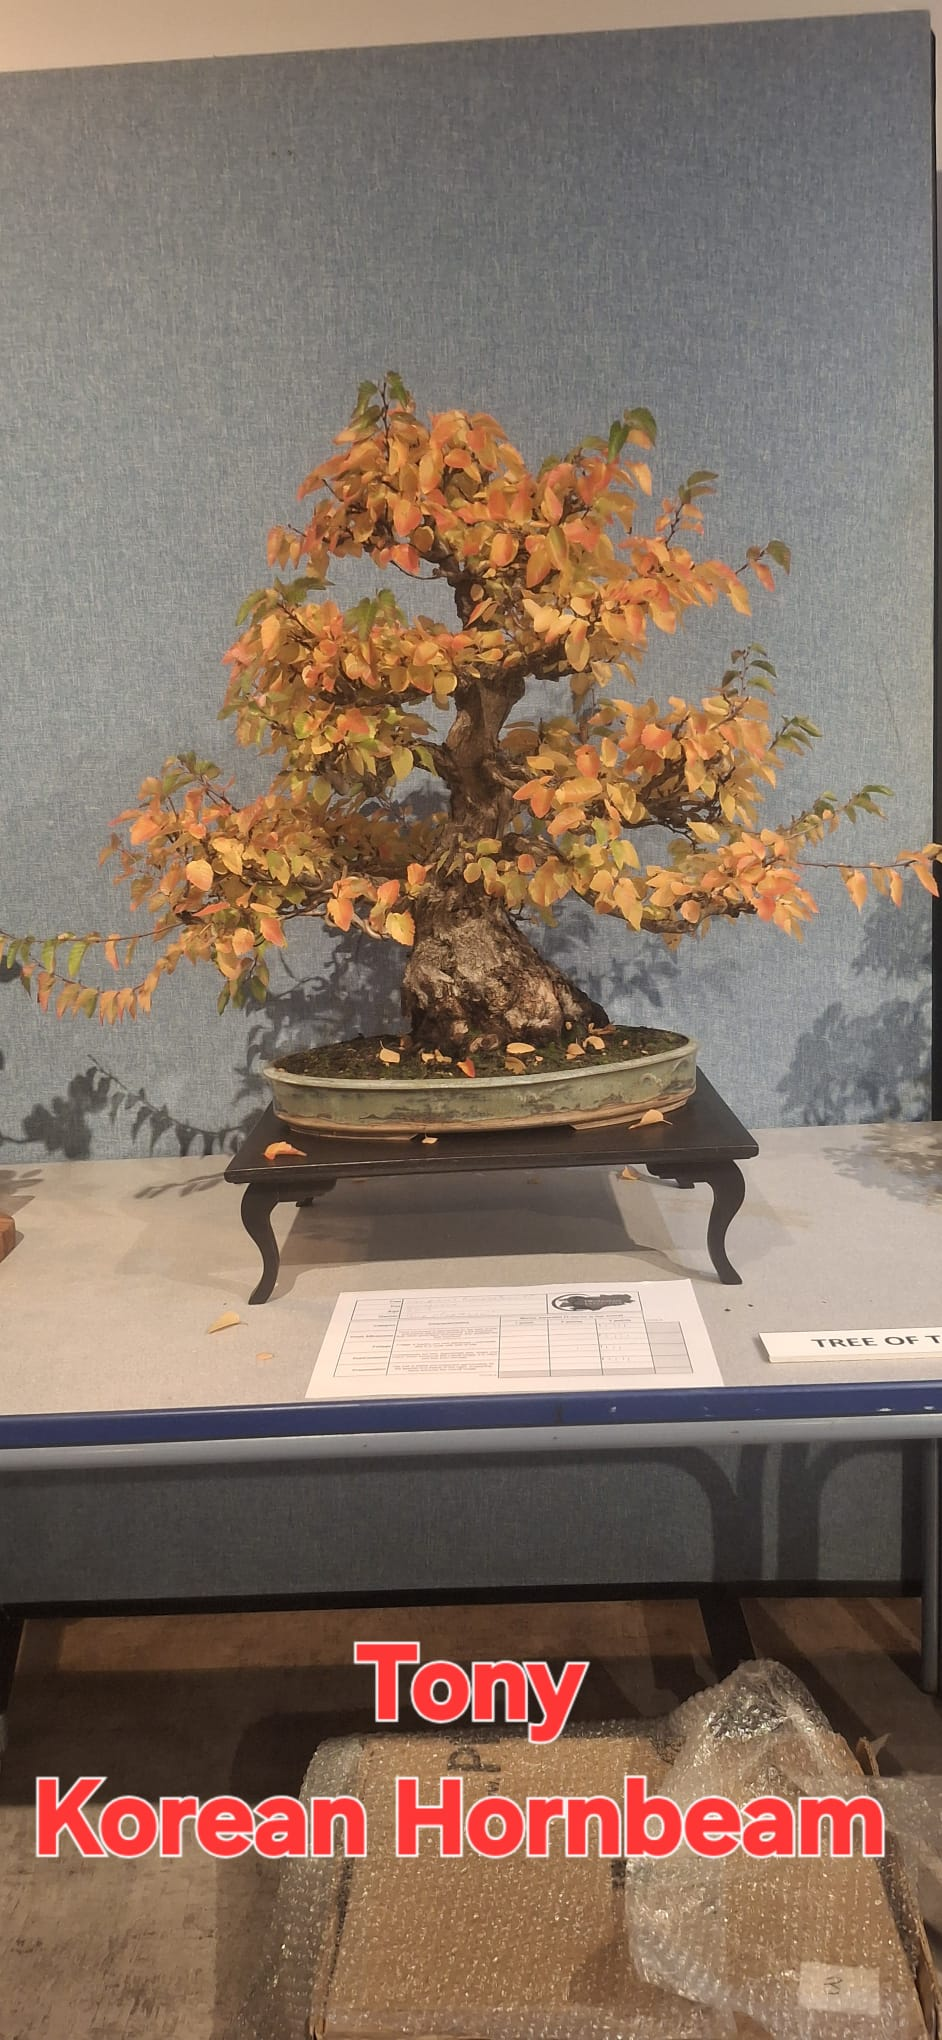
\includegraphics[angle=0,origin=c,width=1.0\textwidth]{2025_10/res/contest_tony_ulatowski_korean_hornbeam}
        \centerline{\emph{Tony Ulatowski's Hornbeam}}
    \end{minipage}\quad
    \begin{minipage}[b]{.275\textwidth}
        
\includegraphics[angle=0,origin=c,width=1.0\textwidth]{2025_10/res/contest_terry_wilson_boston_ivy}
        \centerline{\emph{Terry Wilson's Boston Ivy}}
    \end{minipage}
\end{center}

\begin{center}
    \begin{minipage}[b]{.225\textwidth}
        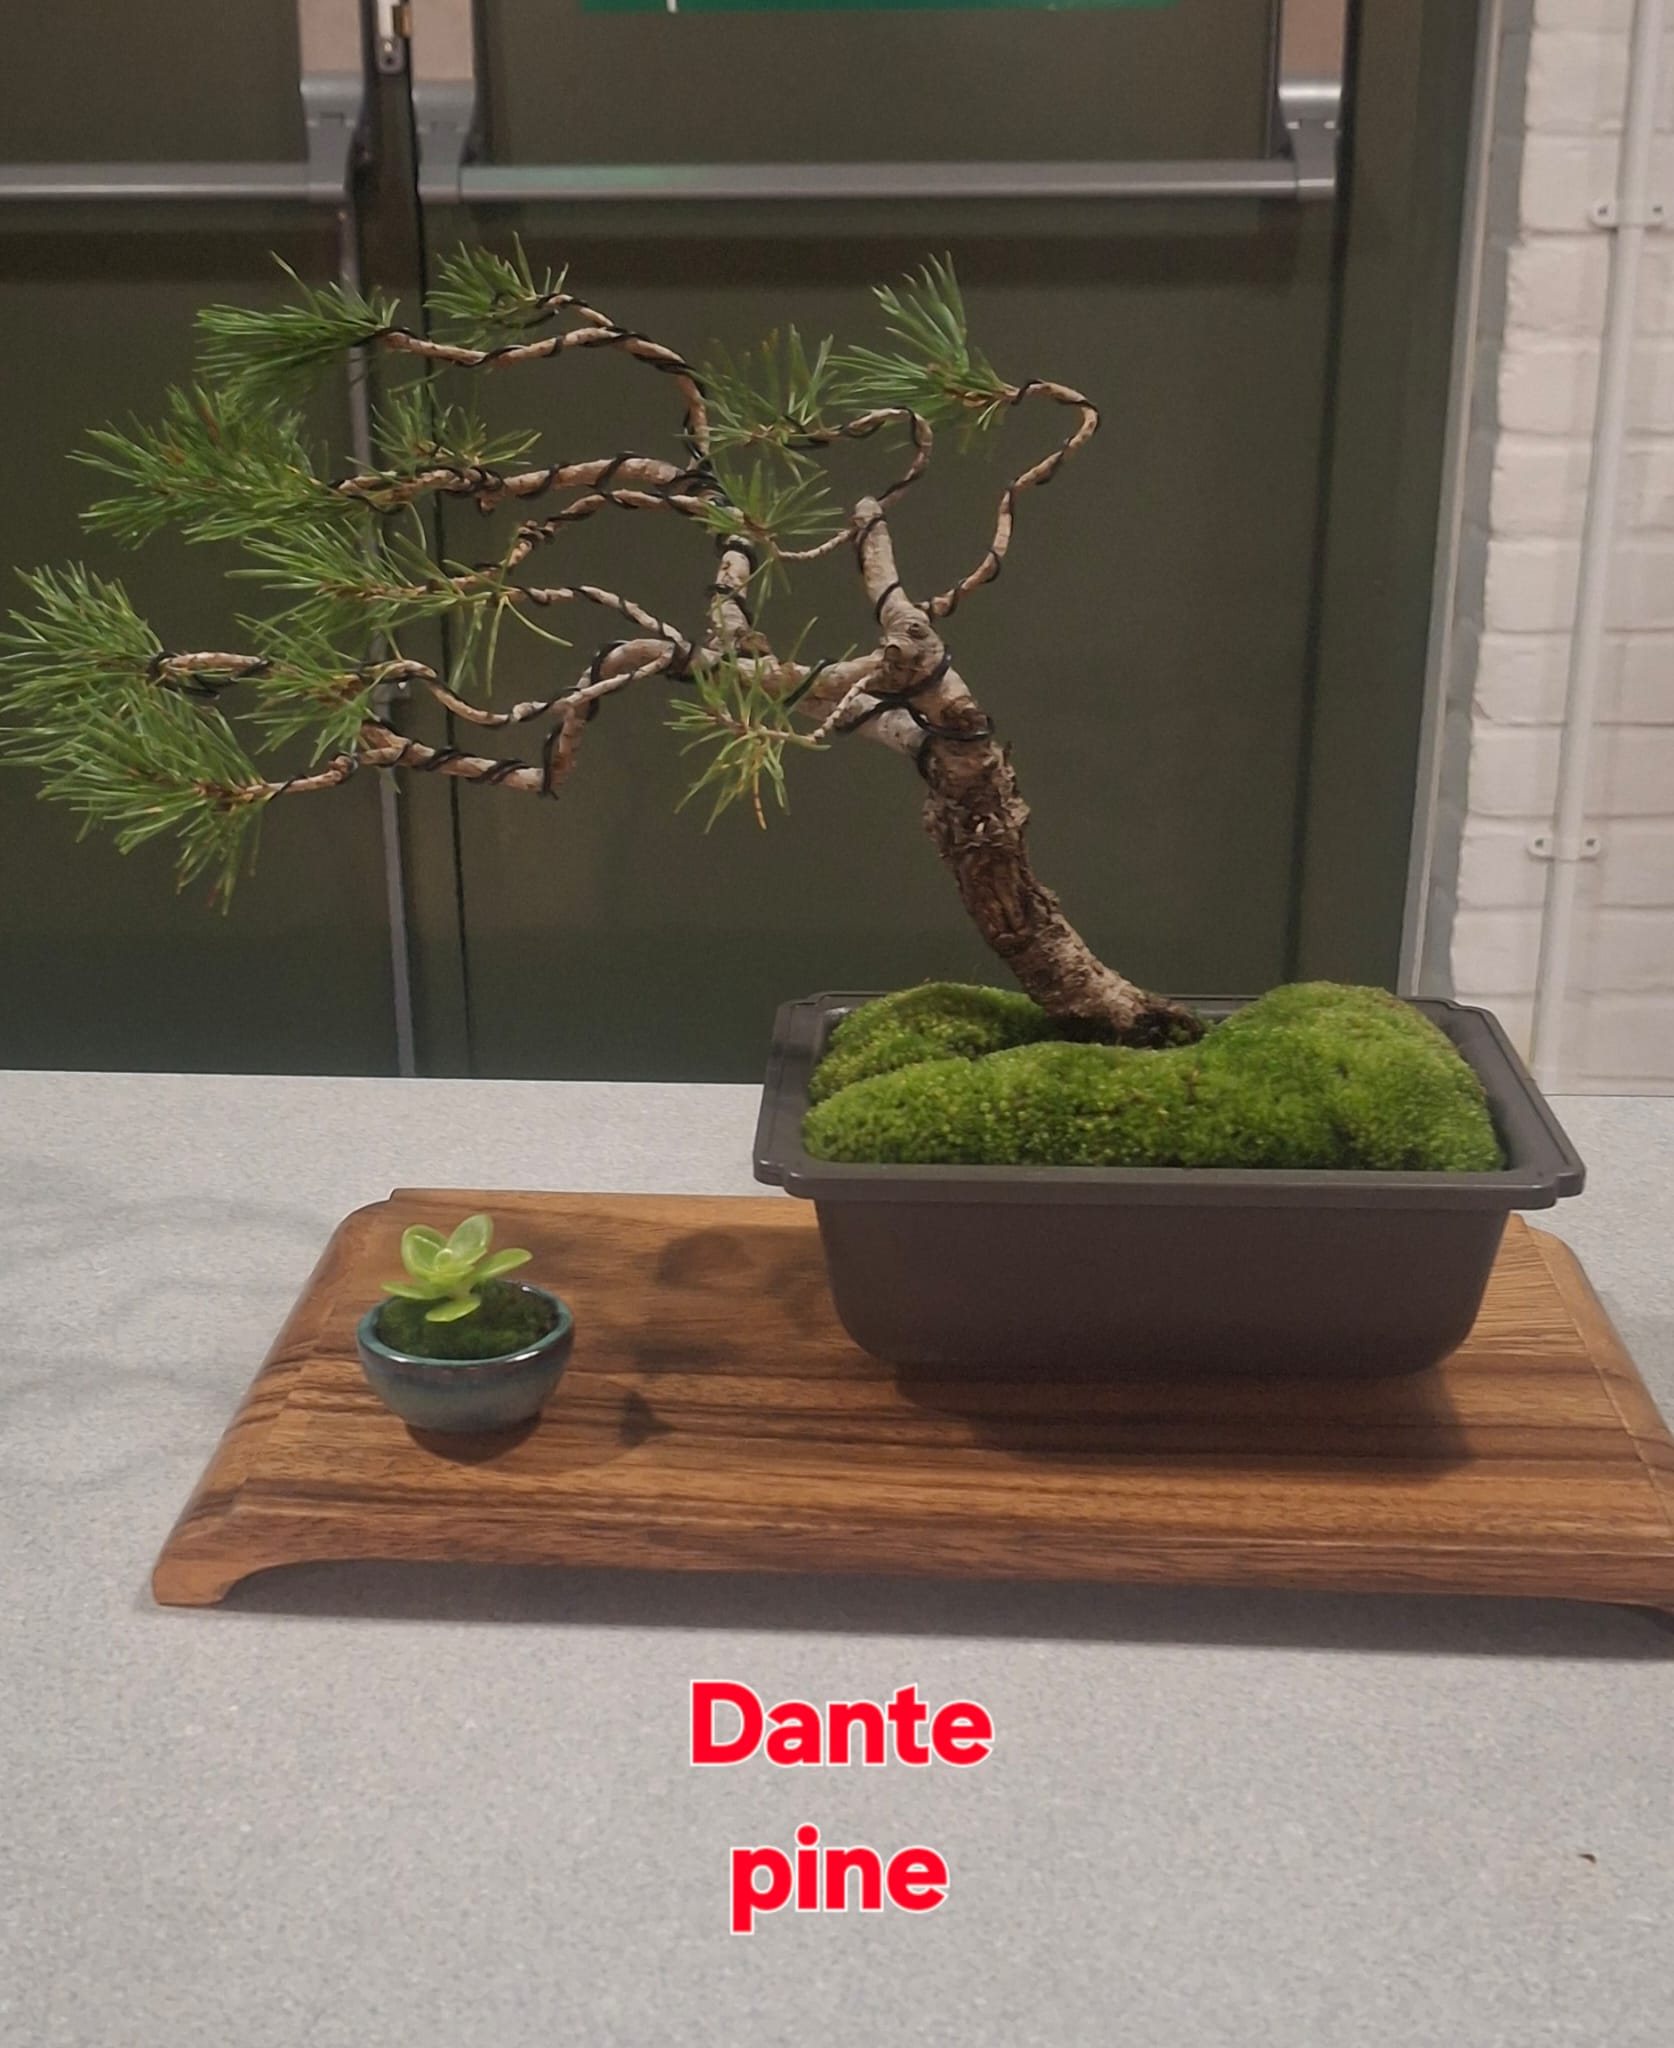
\includegraphics[angle=0,origin=c,width=1.0\textwidth]{2025_10/res/novice_dante_martini_pine}
        \centerline{\emph{Dante Martini's Pine}}
    \end{minipage}\quad
    \begin{minipage}[b]{.225\textwidth}
        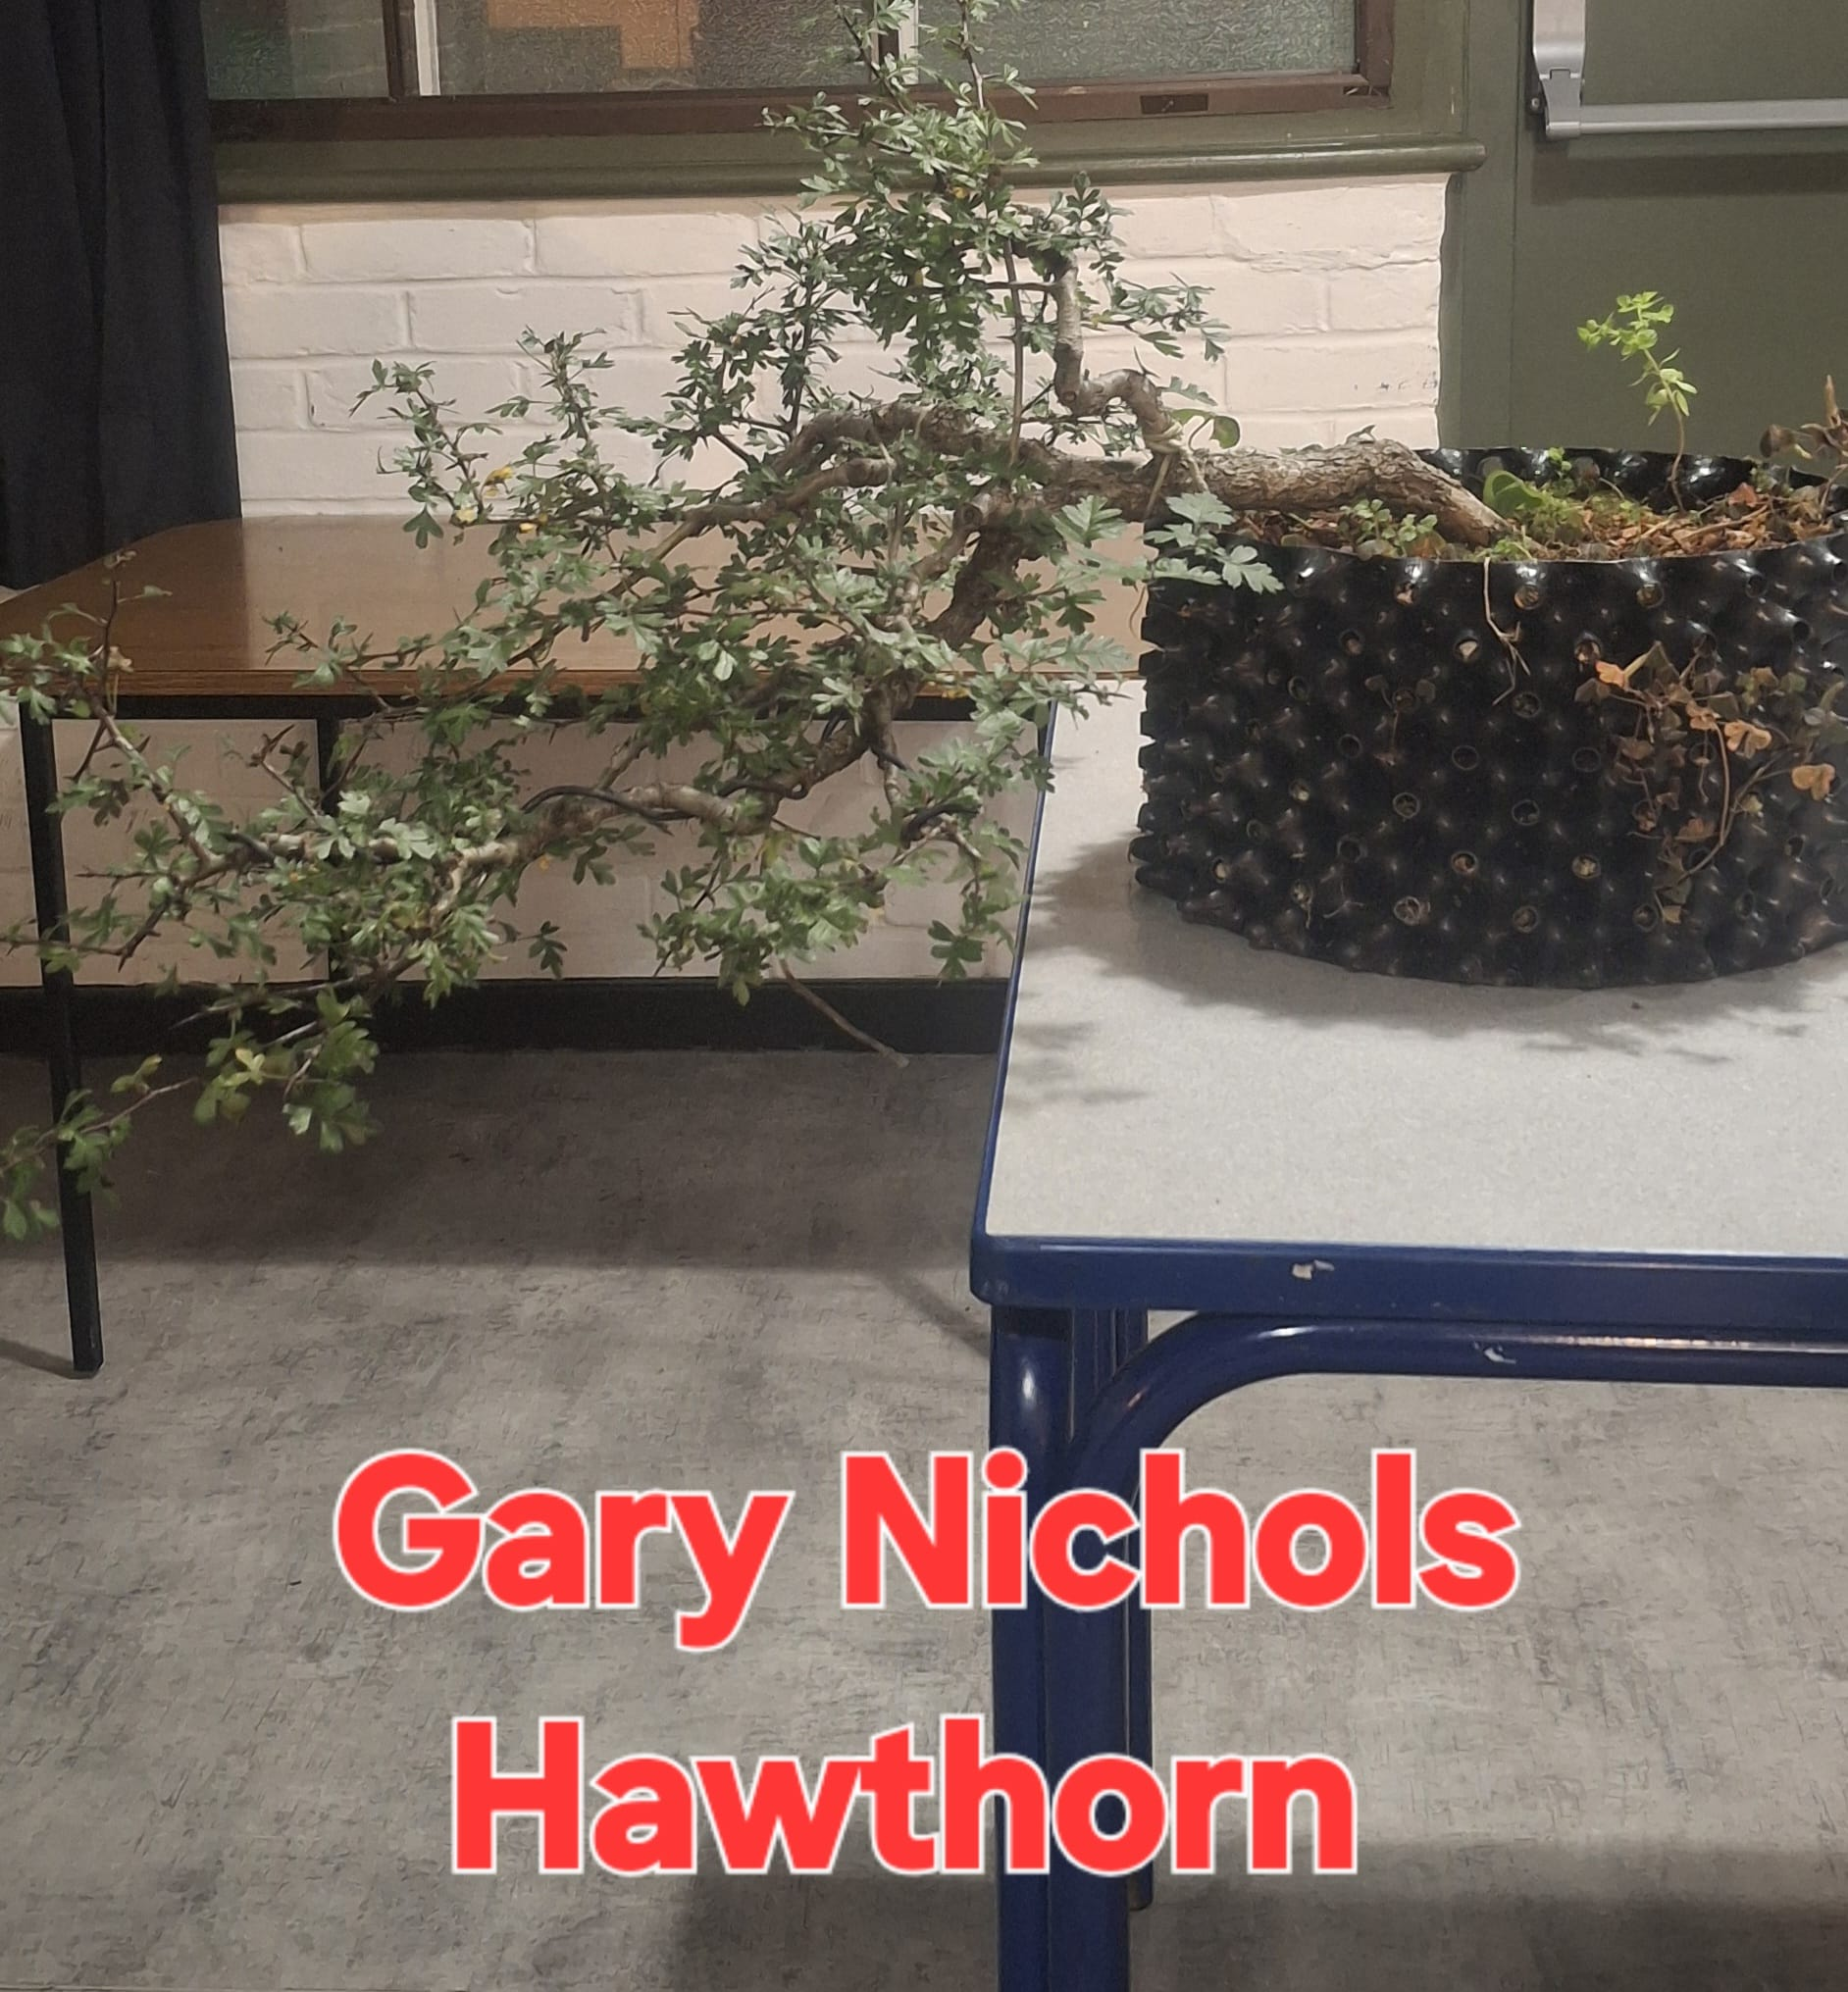
\includegraphics[angle=0,origin=c,width=1.0\textwidth]{2025_10/res/novice_gary_nichols_hawthorn}
        \centerline{\emph{Gary Niochols' Hawthorn}}
    \end{minipage}\quad
    \begin{minipage}[b]{.225\textwidth}
        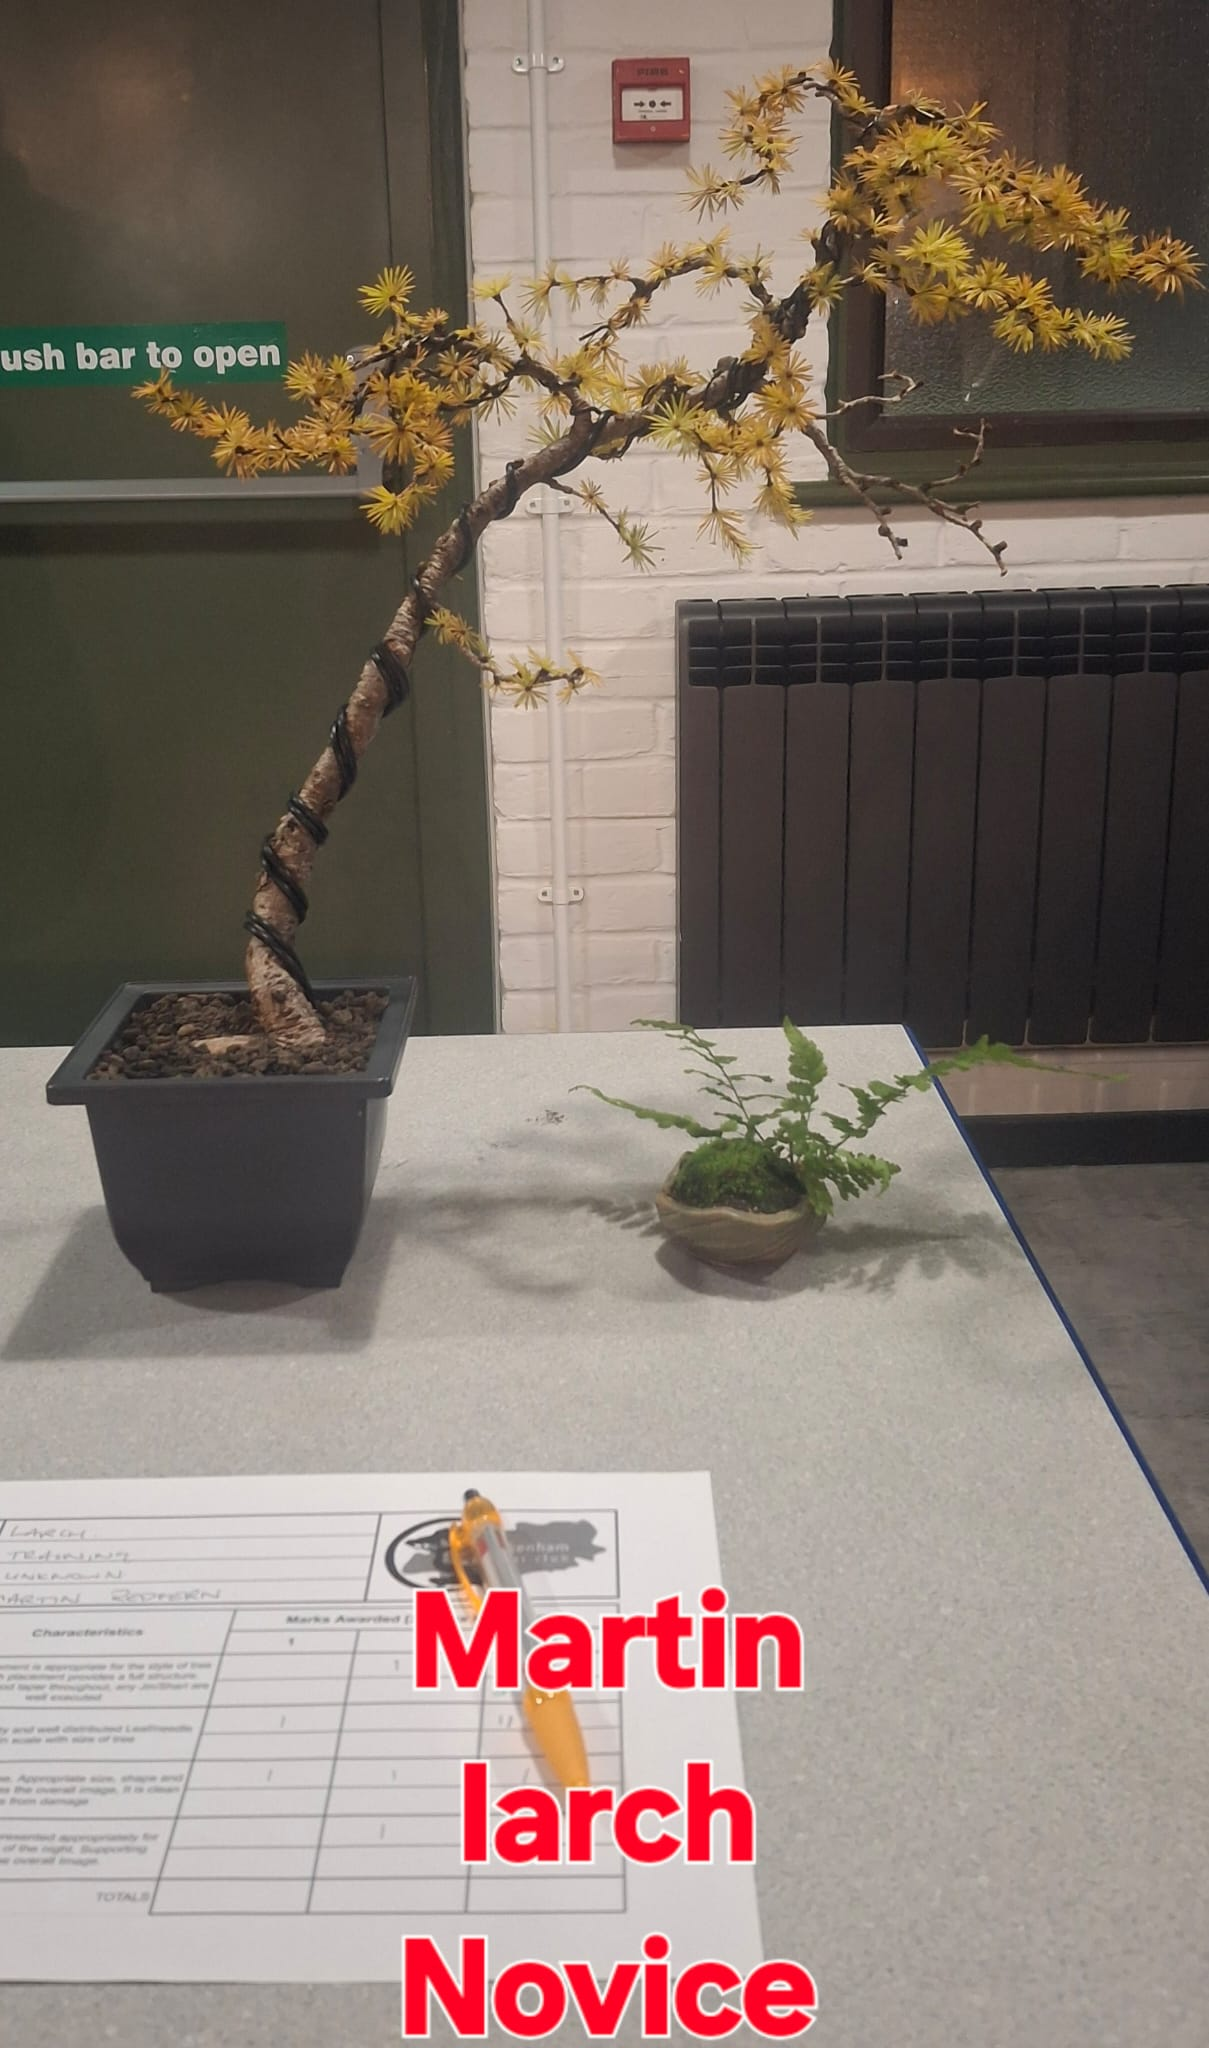
\includegraphics[angle=0,origin=c,width=1.0\textwidth]{2025_10/res/novice_marting_redfern_larch}
        \centerline{\emph{Martin Redfern's Larch}}
    \end{minipage}\quad
    \begin{minipage}[b]{.225\textwidth}
        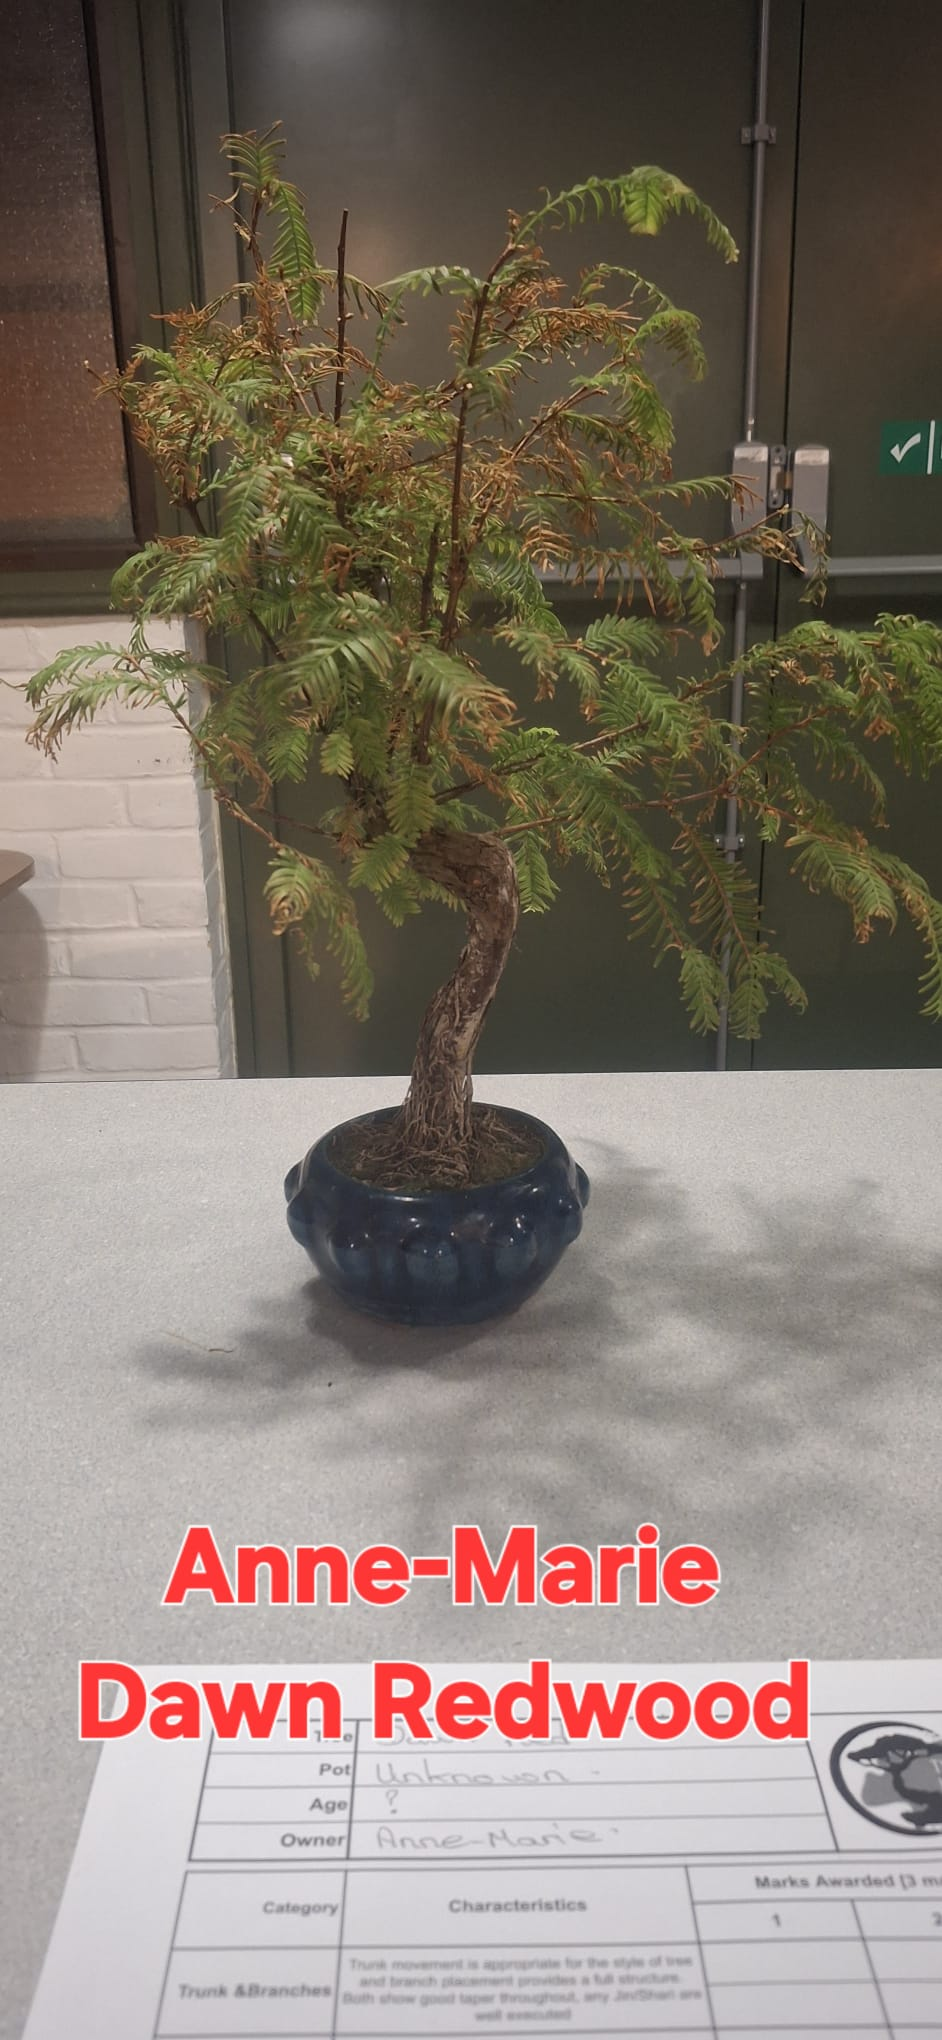
\includegraphics[angle=0,origin=c,width=1.0\textwidth]{2025_10/res/novice_anne_marie_weir_dawn_redwood}
        \centerline{\emph{Anne\--Marie Weir's Redwood}}
    \end{minipage}
\end{center}
\clearpage

\begin{multicols}{2}

